\section{Introduction, Statistical Mechanics Review}

\subsection{Overview}
This course centers around critical phenomena and phase transitions (primarily in magnetic systems/the Ising model) - PHYS 403 is a more comprehensive overview of the field, this is more specialized. We will discuss models that are analytically solvable (or almost), some renormalization group methods, some conformal field theory and the conformal bootstrap method.

We will begin with a review of some basic statistical mechanics. In a nutshell, statistical mechanics is the application of probability theory to a physical system - typically, with a large number of degrees of freedom as this is the limit where the application is useful. Perhaps saying probability theory is a bit reaching, though - the probability involved is pretty minimal (lots of counting, not a ton of measure theory). It is worth noting that (much like other fields of physics) there are very few systems that are analytically solvable; most systems require the application of approximate techniques.

\subsection{Canonical Ensemble}
There are various places to begin this discussion; let's start by discussing the canonical ensemble. Let us consider a physical system, which has an array of possible states. Let us assume that it is characterized by energies $E_a$, and the energy can take up one out of a list of possible values $E_1, E_2, E_3, \ldots$. Given the conservation of energy for a closed system, this is a reasonable way to characterize a state (and given one of our goals of doing thermodynamics with our system, this is a useful quantity). Let us not say too much more about the system - other than perhaps the fact that the energy has a lower bound (but not necessarily an upper bound), and that the energies are ordered. Further, for now let us assume that the energies are discrete - this is of course not true in general (there exist systems for which energy is a continuum, and there we will have to use some kind of binning procedure), but let us assume this simplification for now.

So, how do we make the canonical ensemble? We take $\N$ copies of the system, with various energies, so that $\mathcal{E} = \sum_{i=1}^{\N} E_i$ is the total energy. The $\N$ copies of the system are weakly coupled to each other. This means that energy can flow between the systems, but also that (since the coupling is weak) when we calculate the total energy we can neglect the interaction energies between the systems. In other ensembles, other things that are not the energy can be exchanged (e.g. particles in the grand canonical ensemble).

\begin{figure}[htbp]
    \centering
    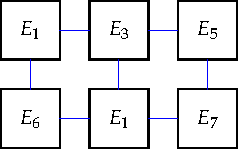
\includegraphics[]{Images/fig-canonicalensemble.pdf}
    
    \caption{Cartoon of the Canonical Ensemble - we consider $\N$ ($= 6$ here) copies of a system, and weakly couple them such that they can exchange energy. Due to artistic constraints the couplings are only drawn for nearest neighbours, but in reality all the systems are coupled to each other.}
    \label{fig-canonicalensemble}
\end{figure}

In state of the ensemble is specified by the number of systems with a given energy, i.e. there are $n_1$ systems with energy $E_1$, $n_2$ systems with energy $E_2$, and so on. The total energy is then given by:
\begin{equation}
    \mathcal{E} = \sum_{a} n_a E_a
\end{equation}
and the number of systems in the ensemble is given by:
\begin{equation}
    \N = \sum_a n_a
\end{equation}

\subsection{Fundamental Postulate - Equal a Priori Probability}
To do statistical mechanics, we require a fundamental postulate - namely, an ``equal a priori probability''. This says that every distinct configuration of the ensemble is equally likely, subject to the total energy and number constraints. Physically, this means that the systems in the ensemble in time are flipping around the possible energy states (in a way that the total energy of the ensemble is conserved). The most probable configuration is the state in which the system spends the most time.

There are other versions of this; we can for example divide a system up in space, and then a spatial average will yield the most probable distribution.

What we look for (since the system visits every possible configuration equally) is the configuration which can be made in the most number of ways. And this is really the only probability theory we have to worry about here; counting up the number of ways to yield a given configuration of the ensemble. So, we ask how many ways are there to make the state $(n_1, n_2, \ldots)$? Let us derive this. Starting with the systems with energy $E_1$, we have:
\begin{equation}
    \N(\N-1) \ldots (\N - n_1 + 1)
\end{equation}
ways to have $n_1$ systems with energy $E_1$ (this is obtained by considering there are $\N$ systems to choose to have energy $E_1$, then $\N - 1$ systems, and so on until all $n_1$ systems have been chosen). But this is overcounting because we don't care about the order, so really we require to divide this by $n_1!$:
\begin{equation}
    \frac{\N(\N-1) \ldots (\N - n_1 + 1)}{n_1!}
\end{equation}
and we continue with $n_2, n_3$ and so on until everything is full:
\begin{equation}
    \frac{\N(\N-1) \ldots (\N - n_1 + 1)}{n_1!} \frac{(\N - n_1) \ldots (\N - n_1 - n_2 + 1)}{n_2!} \ldots = \frac{\N!}{n_1!n_2!\ldots}
\end{equation}
So, the most probable state of the system is that for which the above is maximized; in other words, we maximize it subject to $\sum_{a} n_a = \N$ and $\sum_a n_a E_a = \mathcal{E}$. This is a optimization problem with constraints - this may remind you of Lagrange multipliers which you have seen in classical mechanics. There is an apparent difficulty here in the fact that our numbers are discrete, but we'll get around it. To start, let us take the logarithm of the expression; we can maximize the logarithm of it instead of the original expression, and this is legal as the logarithm is monotonic (this is also a common trick done in machine learning and maximum likelihood estimation). The technique of Lagrange multipliers tells us that the expression of our interest is:
\begin{equation}\label{eq-Lagrangemults}
    \ln(\frac{\N!}{n_1!n_2! \ldots}) + \beta\left(\sum_a n_a E_a - \mathcal{E}\right) + \gamma\left(\sum_a n_a - \N\right)
\end{equation}
it would be nice to be able to use calculus techniques to solve this problem; to this end let us work in the regime of large $\N$ such that we can make the continuum approximation. At first this might seem like a poor assumption; after all after we saturate $\mathcal{E}$ all of the $n_a$s past that point better not be large, but instead zero! To get around this we could assume some kind of cutoff to the energies. Of course there is still a decaying tail to the $n_a$s, but these turn out to not be a problem.

In any case, let us suppose that we can approximate $\N$ large. Then, we can apply Stirling's formula:
\begin{equation}\label{eq-Stirling}
    \ln \N! \approx \N\ln \N - \N.
\end{equation}

\subsection{Interlude - Deriving Stirling's Formula}
We start by writing down an integral expression for the factorial:
\begin{equation}
    \N! = \int_0^\infty dx x^\N e^{-x}
\end{equation}
we solve this via a saddle point technique of replacing the integrand with its maximum value; taking the derivative of the integrand and setting it to zero, we have:
\begin{equation}
    \N x^{\N-1}e^{-x} - x^\N e^{-x} = 0
\end{equation}
which is maximized at $x = \N$. so, the approximate value of the factorial is:
\begin{equation}
    \N! \approx \N^\N e^{-\N}
\end{equation}
and taking logarithms we get Eq. \eqref{eq-Stirling}. This technique also gives us a way of considering corrections to Stirling's formula by considering $x$ near $\N$ (the next order corrections to $\ln \N!$ are $O(\log \N)$, for example).

Another quick and dirty way to derive the formula (that doesn't give a nice way to study corrections, but gives us the leading terms that we want). Using the definition of the factorial and laws of logarithms, we have:
\begin{equation}
    \ln \N! = \sum_{j=1}^\N \ln j
\end{equation}
now approximating the sum as an integral:
\begin{equation}
    \ln\N! \approx \int_1^\N dj \ln j = \N\ln\N - \N + 1
\end{equation}
in the large $\N$ limit we may neglect the $+1$, and we (again) obtain Stirling's formula.

\subsection{Deriving the Boltzmann Distribution}
Applying Stirling's Formula, Eq. \eqref{eq-Lagrangemults} becomes:
\begin{equation}
    \N\ln\N - \N - \sum_a(n_a \ln n_a - n_a) + \beta(\sum_a E_a n_a - \mathcal{E}) + \gamma(\sum_a n_a - \N) = \N\left(\sum_a(-\rho_a \ln \rho_a) + \beta(\sum_a \rho_a E_a - U) + \gamma(\sum_a \rho_a - 1)\right)
\end{equation}
where we define $\rho_a = \frac{n_a}{N}$ and the second expression follows by algebra. Now, since $\rho_a$ varies slowly, we may use techniques of calculus and take a derivative of the above expression and set it to zero. The $\rho_a$ equation reads:
\begin{equation}
    -\ln \rho_a - 1 + \beta E_a + \gamma = 0
\end{equation}
we also take derivatives by $\beta, \gamma$ and set them to zero (as we do with the Lagrange multiplier technique):
\begin{equation}
    \sum_a \rho_a E_a = U
\end{equation}
\begin{equation}
    \sum_a \rho_a = 1
\end{equation}
Let us rearrange the first equation, which has solution:
\begin{equation}
    \rho_a = e^{\beta E_a + \gamma - 1}
\end{equation}
we don't solve the second one, but the third one gives us:
\begin{equation}
    \rho_a = \frac{e^{\beta E_a}}{\sum_a e^{\beta E_a}}
\end{equation}
Note that the $e^{\gamma - 1}$ goes away when we solve the third equation. It would have been wise to choose $\beta$ with the other sign to start with. As we have derived things here, things only make sense if $\beta < 0$. We note that we have derived the ever-famous partition function:
\begin{equation}
    Z = \sum_a e^{\beta E_a}
\end{equation}

So, we have solved for the most likely distribution $\rho_a$; this is the known as the ``Boltzmann distribution''. We have not solved explicitly for $\beta$, but the second equation is formally unsolvable, and we will find a nice interpretation for $\beta$ anyway (as the familiar $\beta = -\frac{1}{k_B T}$). 

\subsection{Example: Two-level system}
We really have not done any physics at all here; but, we have completely generically found the most probable distribution. Let us try applying this to a two-level system and see how good our result is. Particles can have two (spin) states, $\uparrow$ and $\downarrow$. Let us assume we have two particles, and let us assume all orientations of the spins have the same energy. We can just enumerate all the states, and characterize the system by the net magnetization $m = \# \uparrow - \# \downarrow$. We have the four states $\uparrow \uparrow$ with $m = 2$, $\downarrow \downarrow$ with $m = -2$, $\uparrow\downarrow$ and $\downarrow \uparrow$ with $m = 0$. Here, the technique of most probable distribution is quite poor - there is a very good probability that the system is actually ferromagnetic (in fact half of the time) even though the most probable distribution is that the system is unmagnetized. However, we are able to see that unmagnetized is the most probable distribution, and in fact this is true for any number of particles.

So, let's consider generically $N$ particles (note - let us assume that $N$ is even so we can avoid frustration; if $N$ is odd then there exists no configuration with zero magnetization). With $N$ particles, the number of states with $n$ spins up (from which we can obtain the magnetization as $m = n - (N - n) = 2n - N$) is $\frac{N!}{n!(N-n)!}$ of $2^n$ total possible states.

If we then plot $\ln \frac{N!}{n!(N-n)!}$ (making the continuum approximation), we find:

\begin{figure}[htbp]
    \centering

    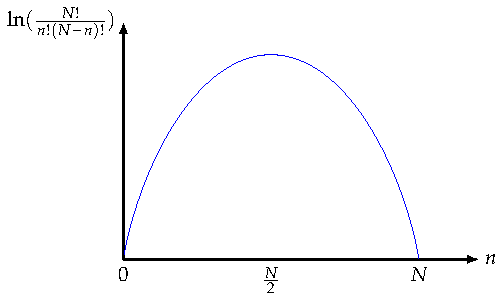
\includegraphics[]{Images/fig-TLSstatecounting.pdf}
    
    \caption{Plot of (continuum approximation) $\ln\frac{N!}{n!(N-n)!}$ as a function of number of spin-up spins $n$. We see the maximum at $n = N/2$ (zero magnetization).}
    \label{fig-TLSstatecounting}
\end{figure}

so indeed the state with $n = N/2$ spins up (and $n = N/2$ spins down) - the state with total magnetization $m = 0$ is the most probable state. It is also valuable to ask what fraction of the total number of states is the most likely distribution. This is simply obtained by taking the number of states with $n = N/2$ and dividing by the total $2^n$:
\begin{equation}
    \frac{N!}{(N/2)!(N/2)!} \frac{1}{2^{n}}
\end{equation}
We find that (using Stirling's formula that):
\begin{equation}
    \ln( \frac{N!}{(N/2)!(N/2)!} \frac{1}{2^{N}}) = 0 + \frac{\ln N}{N}
\end{equation}
so in the $N \to \infty$ limit, $\frac{N!}{(N/2)!(N/2)!} \frac{1}{2^{N}} \approx 1$ to leading order, so the proportion of the most likely distribution to total states of the system is one (with corrections given by the successive terms).